\documentclass[10pt,twocolumn,letterpaper]{article}

\usepackage{cvpr}
\usepackage{times}
\usepackage{epsfig}
\usepackage{graphicx}
\usepackage{amsmath}
\usepackage{amssymb}
\usepackage{mathtools}% Loads amsmath
\usepackage{array}
\usepackage{caption}
\usepackage{float}
\usepackage{multirow}

\graphicspath{{Images/}}
% Include other packages here, before hyperref.

% If you comment hyperref and then uncomment it, you should delete
% egpaper.aux before re-running latex.  (Or just hit 'q' on the first latex
% run, let it finish, and you should be clear).
\usepackage[pagebackref=true,breaklinks=true,letterpaper=true,colorlinks,bookmarks=false]{hyperref}

\cvprfinalcopy % *** Uncomment this line for the final submission

\def\cvprPaperID{****} % *** Enter the CVPR Paper ID here
\def\httilde{\mbox{\tt\raisebox{-.5ex}{\symbol{126}}}}

% Pages are numbered in submission mode, and unnumbered in camera-ready
% \ifcvprfinal\pagestyle{empty}\fi
\begin{document}

%%%%%%%%% TITLE
\title{Image Panoptic Segmentation Challenges using COCO Dataset \\ Project Report : CS 7643}

\author{Anurag Sen, Jie Song, Zhiling Zhou, Zixiang (David) Zhu\\
Georgia Institute of Technology\\
North Ave NW, Atlanta, GA 30332, United States\\
{\tt\small (asen48,jsong407,zhiling\_zhou,zzhu72)@gatech.}
% For a paper whose authors are all at the same institution,
% omit the following lines up until the closing ``}''.
% Additional authors and addresses can be added with ``\and'',
% just like the second author.
% To save space, use either the email address or home page, not both
%\and
%Second Author\\
%Institution2\\
%First line of institution2 address\\
%{\tt\small secondauthor@i2.org}
}

\maketitle
%\thispagestyle{empty}

%%%%%%%%% ABSTRACT
\begin{abstract}
   In this project, we present using various deep learning approaches to perform image panoptic segmentation on MS-COCO dataset. Specifically, we explored both a bottom-up approach (Panoptic DeepLab) and a top-down approach (Panoptic FPN) for image panoptic segmentation tasks. We experimented with various modifications to the existing state-of-the-art models and discovered promising results. 
\end{abstract}

%%%%%%%%% BODY TEXT
\section{Background}

% (5 points) What did you try to do? What problem did you try to solve? Articulate your objectives using absolutely no jargon. 
% (5 points) Who cares? If you are successful, what difference will it make? 

Traditionally, there are two main categories of image segmentation tasks that are widely adopted by many applications: image instance segmentation \cite{hafiz2020survey} and image semantic segmentation \cite{asgari2021deep}. Instance segmentation detects and delineates each distinct object of interest appearing in an image, while semantic segmentation assigns each pixel in an image a class label that it represents. In recent years, image panoptic segmentation has emerged as a new category of image segmentation task that combines both instance segmentation and semantic segmentation \cite{elharrouss2021panoptic}. Specifically, panoptic segmentation generates an output that not only tells which pixels represent each individual object of interest (things) but also assigns a class label to the background pixels (stuff) (Figure \ref{fig:segmentation_types}). Panoptic segmentation has gained greater popularity in the past few years. One application that heavily leverages panoptic segmentation is self-driving cars, where the software needs to distinguish objects (persons, other cars, traffic lights, etc.) from surroundings (road, pavement, sky, etc.) in camera images \cite{behley2021benchmark}. Another application of panoptic segmentation is in medical imaging of tumor cells, where both the tumor instances and the amorphous regions help shape the context of the disease \cite{zhang2018panoptic,cha2021panoptic}.


\begin{figure}[htbp]
\centering
\fbox{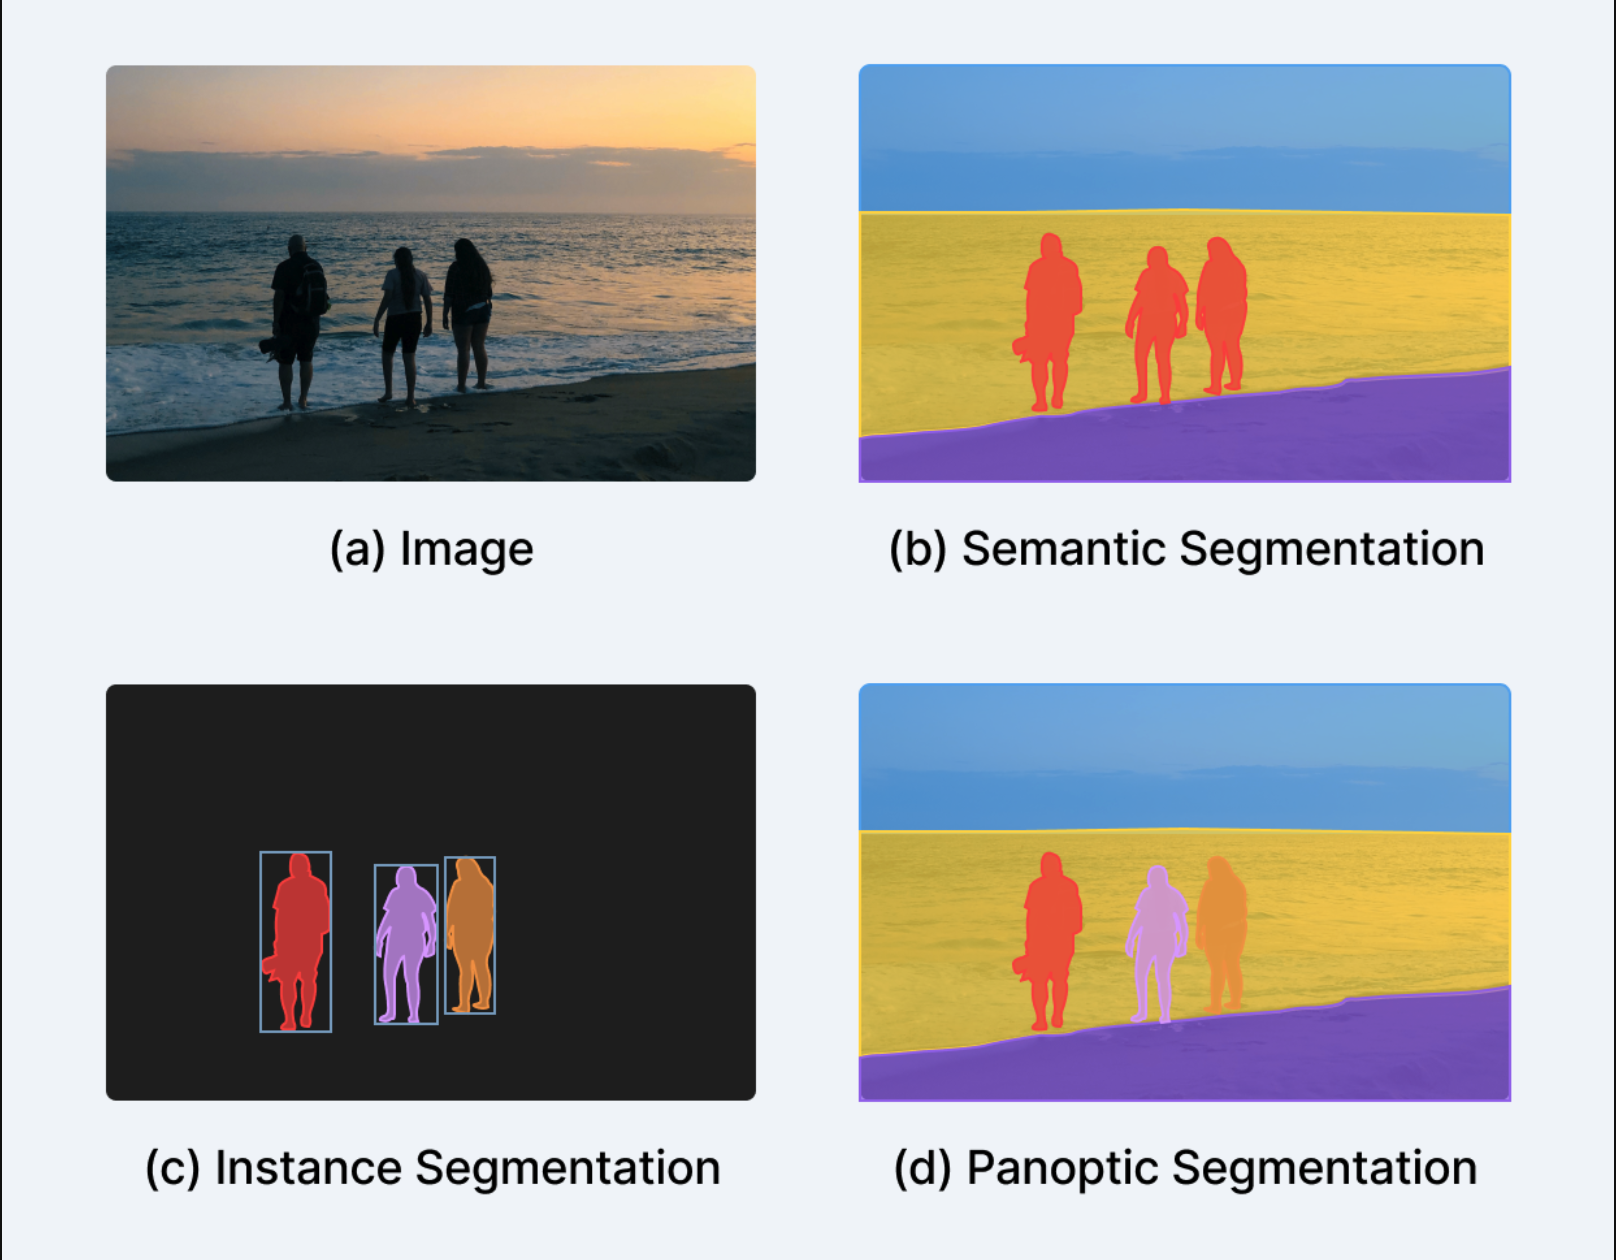
\includegraphics[width=8cm, height=6.5cm]{latex/Images/panoptic_seg.png}}
\caption{Types of image segmentation tasks}
\label{fig:segmentation_types}
\end{figure}

\paragraph{Challenges with Panoptic Segmentation} It has been widely recognized that there are two main challenges in image panoptic segmentation when using Deep Convolutional Neural Network: 1) reduced feature resolution caused by consecutive pooling operations or convolution striding, and 2) the existence of objects at multiple scales in image.

% % (5 points) How is it done today, and what are the limits of current practice?

\paragraph{Panoptic FPN} is a panoptic segmentation model that uses feature pyramid network (FPN) as the backbone to perform both instance segmentation and semantic segmentation. Panoptic FPN is a proposal-based architecture, because it performs ROI pooling on top of FPN which are then used by Mask-RCNN for instance segmentation. Panoptic FPN addresses both aforementioned challenges with its FPN architecture, which can be trained to produce high-resolution, rich, multi-scale features for both instance and semantic segmentation branches. The architecture of Panoptic FPN is studied in more detail in Section \ref{sec:panoptic_fpn}.

\paragraph{Panoptic DeepLab} is a proposal-free architecture that directly predicts object center and offsets from feature maps. Panoptic DeepLab addressed the aforementioned two challenges with its Atrous Spatial Pyramid Pooling (ASPP) filters. ASPP and Panoptic DeepLab architecture are discussed in more detail in Section \ref{sec:deeplab}.


\section{Dataset, Library, and Framework}
% (5 points) What data did you use? Provide details about your data, specifically, choose the most important aspects of your data mentioned \href{https://arxiv.org/abs/1803.09010}{here}. You don’t have to choose all of them, just the most relevant.

\paragraph{Dataset} 
We used COCO 2017 image segmentation dataset to train and test our panoptic segmentation models \cite{lin2014microsoft}. COCO is a large-scale object detection, segmentation, and captioning dataset. The dataset consists of 118k training images and 5k validation images. There are a total of 133 classes that were annotated for panoptic segmentation tasks.

\paragraph{Library and Framework}
We used Detectron2 as the main library to build, train, and test our panoptic segmentation models. Detectron2 is a Pytorch-based library that provides state-of-the-art detection and segmentation algorithms, including Panoptic FPN and Panoptic DeepLab methods for panoptic segmentation \cite{wu2019detectron2}. In this project, we made our own modifications to these algorithms and evaluated their performance on the COCO dataset.

%-------------------------------------------------------------------------
%------------------------------------------------------------------------
\section{Panoptic DeepLab}
\label{sec:deeplab}

Panoptic DeepLab is a single-shot, bottom-up panoptic segmentation method that adopts dual-ASPP and dual-decoder structures for semantic and instance segmentation. The semantic segmentation branch closely resembles to DeepLabV3 (an architecture dedicated for semantic segmentation), while the instance segmentation branch performs class-agnostic object detection through an object center heatmap head and an object center offset head.

Inspired from DeepLabV3, Panoptic DeepLab uses Atrous Spatial Pyramid Pooling (ASPP) to resample feature maps at multiple rates prior to decoder convolutions. Specifically, ASPP is able to probe the original feature map with multiple filters that have complementary fields of view, through which objects as well as their contexts are captured at multiple scales. 

Panoptic DeepLab uses ResNet as its backbone encoder (feature extractor). The output of the last stage of ResNet is fed into two ASPP layers in parallel, which are used to extract denser feature maps at different scales. From there the output of one ASPP is fed into a semantic segmentation decoder, while the output of the other ASPP is fed into an instance segmentation decoder. Feature maps in both decoders undergo an upsampling process, after which the outputs of both decoders are fused together into one segmentation output. 

Parts of Panoptic DeepLab with learned parameters are: ResNet encoder (convolutional layers), ASPP heads (layers of ASPP filters), semantic and instance segmentation decoders (which incorporates convolutional layers with upsample pooling). The post-processing stage where semantic and instance segmentation outputs are fused does not have learned parameters.

Panoptic-DeepLab is trained with three loss functions: 1) weighted bootstrapped cross entropy loss for semantic segmentation head; 2) MSE loss for center heatmap
head; and 3) L1 loss for center offset head. The final loss L is computed as follows.
\[
L = \lambda_{sem} L_{sem} + \lambda_{heatmap} L_{heatmap} + \lambda_{offset} L_{offset}
\]

\subsection{Approach}

% (10 points) What did you do exactly? How did you solve the problem? Why did you think it would be successful? Is anything new in your approach? 
% (5 points) What problems did you anticipate? What problems did you encounter? Did the very first thing you tried work? 
% \textbf{Important: Mention any code repositories (with citations) or other sources that you used, and specifically what changes you made to them for your project. }

A state-of-the-art Panoptic DeepLab model is already made available in the Detectron2 library. However because the default Panoptic DeepLab model was heavy to train, several exploratory modifications were made to the default model with the hope that some of them can make the model be trained reasonably well with fewer iterations. 

\paragraph{Freezing Pre-trained ResNet Backbone at Different Stages} The default Panoptic DeepLab model uses an ImageNet pre-trained ResNet-50 as its backbone encoder, but the default model does not freeze any ResNet stages during COCO training. In our experiments, we explored freezing different stages of pre-trained ResNet backbone, with the hope that doing so would reduce the number of parameters to train and therefore can result in faster model parameter convergence.

\paragraph{Using Pre-trained ResNet-101 as Backbone} We experimented with using a pre-trained ResNet-101 as the backbone encoder instead of the default ResNet-50. We did this exploration with the hope that a richer ResNet as a feature extractor can feed to ASPP with better feature representations that can provide more useful contexts for decoders to perform semantic and instance segmentation.

\paragraph{Using Single ASPP Head} The default Panoptic DeepLab model has dual ASPP heads. Because ASPP is responsible for extracting features and contexts from the input feature map with different fields of view, we were hoping that both semantic and instance segmentation decoders can share the same features extracted by a single ASPP head, which in turn could reduce the number of parameters learned by DeepLab model and make the model converge faster.

\paragraph{Using Different ASPP Dilation Rates} In the default DeepLab model, the three ASPP layers in each head have dilation rates of 6, 12, and 18, respectively. Because the dilation rate controls how big ASPP fields of views are, this configuration is critical to the performance of DeepLab. We explored changing ASPP dilation rates to different values in order to evaluate the effect of ASPP fields of view on the performance of Panoptic DeepLab.


\subsection{Data Pre-Processing, Training and Evaluation Procedures} 

\paragraph{Data Pre-Processing} Panoptic DeepLab models implemented by Detectron2 expect input as a batch of 3-channel RGB images together with their corresponding 1-channel annotations images, where each pixel in the annotations image represents the class ID that the corresponding pixel in input image represents. All input images are re-sized to a fixed size so large input images can fit into memory. COCO dataset does not provide the 1-channel annotations images, but Detectron2 provides a tool to convert COCO-style JSON annotations into 1-channel annotations images.

\paragraph{Training Procedure} Each variant of Panoptic DeepLab model was trained on the COCO 2017 training dataset with panoptic segmentation annotations. All models were trained with a learning rate of 0.0025, using Adam optimizer with momentum of 0.9 to perform gradient descent.

\paragraph{Model Evaluation}
During inference time, for each input image, the output of Panoptic DeepLab is a 1-channel annotation image of the same size as the input image, where each pixel value in the output image is the class label ID represented by the corresponding input image pixel at that position.

In order to evaluate the performance of segmentation results, a Panoptic Quality (PQ) score of segmentation output with respect to the ground truth annotations was calculated for each test image. We evaluated each model with its average PQ score produced from all testing images. A model that produces output segmentations with higher PQ scores is regarded to have better performance than a model with lower PQ scores.

PQ score is a combination of Segmentation Quality score (SQ) and Recognition Quality score (RQ). SQ evaluates how closely output segments are matched with their ground truths. RQ is a combination of precision and recall, which attempts to identify how effective the model is at getting a prediction right.

\[
  PQ = 
    \underbrace{\frac{\sum\nolimits_{(p, g) \in TP} IOU_{(p, g)}}{|TP|}}_\text{segmentation quality (SQ)} \times 
    \underbrace{\frac{|TP|}{|TP| + \frac{1}{2}|FP| + \frac{1}{2}|FN|}}_\text{recognition quality (RQ)}
\]
where~$p$ is prediction output,~$g$ is ground truth annotations

\subsection{Experiments and Results}

% (10 points) How did you measure success? What experiments were used? What were the results, both quantitative and qualitative? Did you succeed? Did you fail? Why? Justify your reasons with arguments supported by evidence and data.

% \textbf{Important: This section should be rigorous and thorough. Present detailed information about decision you made, why you made them, and any evidence/experimentation to back them up. This is especially true if you leveraged existing architectures, pre-trained models, and code (i.e. do not just show results of fine-tuning a pre-trained model without any analysis, claims/evidence, and conclusions, as that tends to not make a strong project). }


% |        |  PQ   |   SQ   |   RQ   |  #categories  |
% |:------:|:-----:|:------:|:------:|:-------------:|
% |  All   | 6.351 | 44.339 | 8.523  |      133      |
% | Things | 4.259 | 43.053 | 5.773  |      80       |
% | Stuff  | 9.510 | 46.279 | 12.673 |      53       |
\begin{table}[h!]
\begin{center}
\begin{tabular}{ || m{3em} | m{1cm}| m{1cm} | m{1cm} || } 
  \hline
   & PQ & SQ & RQ \\ 
  \hline
  All & 6.351 & 44.339 & 8.523 \\ 
  \hline
  Things & 4.259 & 43.053 & 5.773 \\ 
  \hline
  Stuff & 9.510 & 46.279 & 12.673 \\ 
  \hline
\end{tabular}
\caption{PQ, SQ, and RQ scores of Default Panoptic DeepLab (after 10k iterations).}
\label{tab:deeplab_default}
\end{center}
\end{table}


\subsubsection{Freezing Pre-trained ResNet at Different Stages}

We chose to freeze the first 2, 4, and all 5 stages of pre-trained ResNet. Our experiment shows that with just the first 2 stages of pre-trained ResNet frozen, the Panoptic DeepLab model was able to yield a higher PQ score as compared to the default model where all stages of ResNet were learned (8.06 vs. 6.35). In addition, we also saw that freezing the first 4 stages of pre-trained ResNet resulted in an even better PQ score (16.01). This score is also higher than if all 5 stages of ResNet were frozen (14.85).

The experiment result matches with our earlier hypothesis: freezing some lower-level feature extractors in ResNet and only performing fine-tuning in other parts can make parameters in Panoptic DeepLab model converge faster. This is because freezing lower-level convolutional layers essentially reduces the number of parameters to be learned during training with new data.

Another finding is that not freezing the last stage of ResNet can result in better performance than if all ResNet stages were frozen. This is likely because the last few layers of feature extractor (ResNet) are of greater importance to ASPP because ASPP is built directly on top of feature maps generated by the last stage of ResNet; therefore training the last few layers of ResNet together with ASPP and subsequent decoders would tend to make the gradient of weights w.r.t. loss in ASPP be smoother as opposed to freezing the weights of last stage of ResNet.


\begin{table}[htbp]\centering
\begin{tabular}{ || m{5em} | m{4em} | m{5em}| m{4em} || } 
  \hline
  Freeze up to  & PQ: All & PQ: Things & PQ: Stuff \\ 
  \hline
  N/A & 6.351 & 4.259 & 9.510 \\ 
  \hline
  2\textsuperscript{nd} stage & 8.060 & 6.090 & 11.034 \\ 
  \hline
  4\textsuperscript{th} stage & 16.016 & 15.349 & 17.021 \\ 
  \hline
  5\textsuperscript{th} stage & 14.856 & 13.261 & 17.263 \\ 
  \hline
\end{tabular}
\caption{PQ scores of Panoptic DeepLab with different stages of ResNet frozen (after 10k iterations).}
\label{tab:deeplab_freeze_4}
\end{table}

\subsubsection{Using Pre-trained ResNet-101 as Backbone}

Our experiment shows that ResNet-101-based Panoptic DeepLab was not able to outperform its ResNet-50-based counterpart if only lower layers (stage $\leq$ 2) in pre-trained ResNet were frozen during training. However, if the first 4 stages were frozen, or if all 5 stages were frozen, we saw a significant improvement on PQ scores generated by ResNet-101-based Panoptic DeepLab when compared to the default Panoptic DeepLab with ResNet-50 backbone.

This finding matches with our earlier hypothesis. Specifically, ResNet-101 is a richer model that is able to extract more complex features from input images, but it does so with more parameters to train than ResNet-50. Given to the higher model complexity of ResNet-101, when no stage was frozen or only the first 2 stages were frozen, ResNet-101 weights would take much longer time to converge than ResNet-50, which would result in poorer performance when given a constraint on training iterations. However, if we were only doing fine-tuning (or fine-tuning together with the last stage of pre-trained ResNet), the decoders of DeepLab would be able to leverage the already pre-trained ResNet-101 as a richer feature extractor, and with little additional cost because all weights in lower levels of ResNet-101 were frozen. As a result, the Panoptic DeepLab with ResNet-101 backbone would be able to converge faster than its counterpart with ResNet-50 backbone. 

\begin{table}[htbp]\centering
\begin{tabular}{ || m{5em} | m{4em}| m{5em} | m{4em} || } 
  \hline
Freeze up to & PQ: All & PQ: Things & PQ: Stuff \\ 
  \hline
  2\textsuperscript{nd} stage & 7.250 & 5.340 & 10.132 \\ 
  \hline
  4\textsuperscript{th} stage & 19.484 & 19.691 & 19.172 \\ 
  \hline
  5\textsuperscript{th} stage & 17.731 & 16.865 & 19.037 \\ 
  \hline
\end{tabular}
\caption{PQ scores of custom Panoptic DeepLab with pre-trained ResNet-101 as backbone and different ResNet stages frozen (after 10k iterations).}
\label{tab:deeplab_resnet_101_freeze_2}
\end{table}

\subsubsection{Using Single ASPP Head}

We implemented a custom version of Panoptic DeepLab with single ASPP head. Our experiment shows that Panoptic DeepLab with single ASPP head did not outperform the default model with dual ASPP heads (PQ of 18.10 vs. PQ of 19.48). This finding suggests that instance segmentation and semantic segmentation branches likely require different contextual and
decoding information from ASPP. Our finding matches with the experiment results published in the Panoptic DeepLab paper, which also shows that using dual ASPP heads is able to produce better segmentation outputs than using single ASPP head.

% |        |   PQ   |   SQ   |   RQ   |  #categories  |
% |:------:|:------:|:------:|:------:|:-------------:|
% |  All   | 18.104 | 62.888 | 23.520 |      133      |
% | Things | 18.329 | 68.318 | 23.762 |      80       |
% | Stuff  | 17.763 | 54.693 | 23.154 |      53       |
\begin{table}[htbp]\centering
\begin{tabular}{ || m{5em} | m{4em} | m{5em} | m{4em} ||} 
  \hline
   & PQ: All & PQ: Things & PQ: Stuff \\
  \hline
  Dual ASPP Heads & 19.484 & 19.691 & 19.172 \\ 
  \hline
  Single ASPP Head & 18.104 & 18.329 & 17.763 \\ 
  \hline
\end{tabular}
\caption{PQ scores of Panoptic DeepLab with dual ASPP heads and single ASPP Head. Both models have pre-trained ResNet-101 as backbone, and first 4 stages of ResNet freezed (after 10k iterations).}
\label{tab:deeplab_single_aspp_freeze_2}
\end{table}

\subsubsection{Using Different ASPP Dilation Rates}

We experimented with enlarging and shrinking ASPP fields of view by changing ASPP filters' dilation rates. The results showed that there is no significant change of segmentation performance if ASPP fields of views were shrunk by half, whereas there is a significant drop in performance if ASPP field of view is doubled. 

\begin{table}[htbp]\centering
\begin{tabular}{ || m{6em} | m{4em} | m{5em} | m{4em} ||} 
  \hline
  ASPP Dilation Rates & PQ: All & PQ: Things & PQ: Stuff \\
  \hline
  3,  6,  9  & 19.356 & 19.513 & 19.120 \\ 
  \hline
  6,  12, 18 & 19.484 & 19.691 & 19.172 \\ 
  \hline
  12, 24, 36 & 18.677 & 18.879 & 18.371 \\ 
  \hline
\end{tabular}
\caption{PQ scores of custom Panoptic DeepLab with different ASPP dilation rates. All models have pre-trained ResNet-101 as backbone, and first 4 ResNet stages freezed (after 10k iterations).}
\label{tab:deeplab_small_fov}
\end{table}

\subsubsection{Hyper-parameter Tuning}

From the experiment results shown above, the best Panoptic DeepLab variant when trained with 10k iterations was the one that was based on pre-trained ResNet-101 and had the first 4 ResNet stages frozen. We then performed hyper-parameter tuning on top of this model in order to further improve its performance. 

\paragraph{Increasing Batch Size}
% |        |   PQ   |   SQ   |   RQ   |  #categories  |
% |:------:|:------:|:------:|:------:|:-------------:|
% |  All   | 22.502 | 68.998 | 29.112 |      133      |
% | Things | 23.011 | 71.151 | 29.809 |      80       |
% | Stuff  | 21.734 | 65.749 | 28.060 |      53       |
\begin{table}[htbp]\centering
\begin{tabular}{ || m{5em} | m{4em} | m{5em} | m{4em} ||} 
  \hline
  Batch Size & PQ: All & PQ: Things & PQ: Stuff \\
  \hline
  5 & 19.484 & 19.691 & 19.172 \\ 
  \hline
  8 & 22.502 & 23.011 & 21.734 \\ 
  \hline
\end{tabular}
\caption{PQ scores of custom Panoptic DeepLab with ResNet-101 as backbone, first 4 ResNet stages frozen, trained with batch size of 8 (after 10k iterations).}
\label{tab:deeplab_batch_size_8}
\end{table}

\paragraph{Adding Weight Decay}
We explored adding a small weight decay to the optimizer as a regularization factor, however the resulting models did not show promising improvements in their PQ scores. This is likely because 1) there are already dropout layers incorporated in Panoptic DeepLab and 2) our batch size is small which already has a regularization effect (added noise).


\subsubsection{Other considerations}

As was observed in Figure \ref{fig:panoptic_deeplab_lc}, overall validation loss kept decreasing in an oscillating fashion while training in the first 10k iterations. Therefore we did not observe model overfitting during our training.

\begin{figure}[htbp]
\centering
\fbox{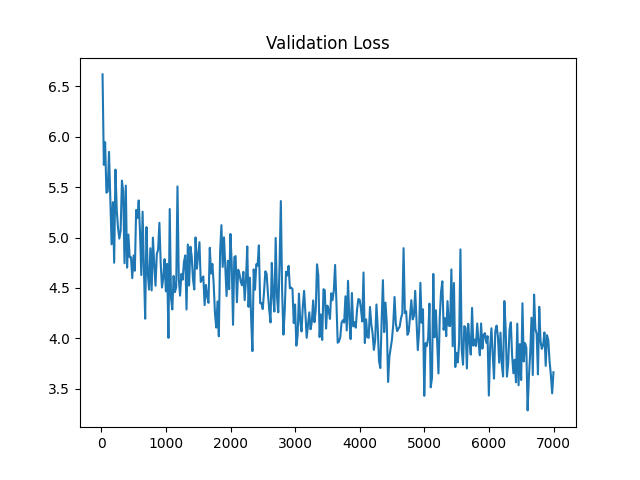
\includegraphics[width=7cm, height=6cm]{latex/Images/panoptic_deeplab_lr.png}}
\caption{Validation loss Ccrve of Panoptic DeepLab training.}
\label{fig:panoptic_deeplab_lc}
\end{figure}

%-------------------------------------------------------------------------
%------------------------------------------------------------------------
\section{Panoptic FPN}
\label{sec:panoptic_fpn}

Panoptic FPN uses FPN (feature pyramid network) as its backbone to generate rich features at different scales. FPN takes a standard network with features at multiple spatial resolutions (i.e., ResNet), and adds a light top-down pathway with lateral connections. Panoptic FPN performs ROI pooling by attaching a Faster R-CNN to FPN. Mask-RCNN is used to generate masks for detected objects from generated ROIs. In order to perform semantic segmentation, Panoptic FPN attaches to FPN with a simple and fast semantic segmentation branch, where each FPN level is upsampled by convolutions and bilinear upsampling until it reaches 1/4 scale, theses outputs are then summed and finally transformed into a pixel-wise output.

Panoptic FPN generates 3 losses in its instance segmentation branch: classification loss, $L_{c}$, bounding box loss, $L_{b}$, and mask loss, $L_{m}$. In addition, Panoptic FPN generates 1 loss in its semantic segmentation branch ($L_{s}$). The semantic segmentation loss is a per-pixel cross entropy loss between the predicted and the ground-truth labels. The final loss is calculated as follows:

\[
L = \lambda_{i} (L_{c} + L_{b} + L_{m}) + \lambda_{s}L_{s}
\]

where ~$\lambda_{i}$ and ~$\lambda_{s}$ are hyper-parameters.

Two major parts of panoptic FPN have learnable parameters. The first part is underlying backbone structures, convolution layers specifically. The second part is the connection layers between feature maps and FPN layers. The model is very complex and due to time constraints, the training loss curves seem to suggest that the model slowly learns even after 270k iterations, so overfitting has yet been identified for now. Major hyperparameters are base learning rate, batch size, and the depth of backbone network, and Adam based optimizers were used. Based the experiment results, batch size and learning rate are two significant hyperparamters affecting performance, but unfortunately due to the limited GPU quota imposed by Google Cloud, we were prevented to apply larger batch sizes (e.g., 16 and plus) because of the memory limits of a single GPU. 

\begin{figure}[htbp]
\centering
\fbox{\includegraphics[width=8cm, height=5.5cm]{latex/Images/fpn.jpg}}
\caption{Panoptic FPN architecture}
\label{fig:fpn}
\end{figure}

\subsection{Approach}

% (10 points) What did you do exactly? How did you solve the problem? Why did you think it would be successful? Is anything new in your approach? 
% (5 points) What problems did you anticipate? What problems did you encounter? Did the very first thing you tried work? 

%\textbf{Important: Mention any code repositories (with citations) or other sources that you used, and specifically what changes you made to them for your project. }

The methods were developed based on Detectron2 library as well. One of the backbones used by the panoptic segmentation tasks is ResNet of various depths. ResNet is applied to extract feature maps of different depths, and FPN is applied to combine these feature maps into a "pyramid" style structure. This structure captures feature information of different resolutions, and its outcomes are further fed into regional proposal algorithms and subsequent semantic and instance segmentation tasks. The selection of backbones therefore determines how feature maps are generated, and this task tends to investigate modified versions of the existing backbone architectures and how the modifications may affect performance, thus deepening our understanding towards panoptic segmentation. Specifically, two modifications were conducted as detailed in the following text (Figure \ref{fig:modifications} in Appendix \ref{app:fpn}). As the fundamental structure of the library is changed, pre-trained weights are no longer usable. We expect that the resulting performance may be below expectation. 

%\begin{figure}[htbp]
%\centering
%\fbox{\includegraphics[width=8.5cm, height=14cm]{latex/Images/mods.jpg}}
%\caption{Modifications to the backbones of a Panoptic FPN architecture}
%\label{fig:modifications}
%\end{figure}

%\subsection{Approach}

\textbf{Two bottleneck layers within a ResNet block}  The purpose of the first modification is to investigate whether a redundant design of the residual block may improve the performance. This minor modification was shown by Figure \ref{fig:modifications}b. The redundant design may provide additional information to a residual block and therefore can enhance the quality of feature maps that will be heavily relied by sebsquent FPN processing and segmentation tasks. 

\textbf{Implementation of a VGG backbone}  The second modification tends to understand how this very classic CNN architecture performs panoptic segmentation tasks (Figure \ref{fig:modifications}a). If the performance is sufficiently sound, the simpler model is always preferred. Figure shows the implementation details of a VGG architecture into a panoptic FPN framework. This VGG architecture is not implemented in the original detectron2 library and built from scratch by us.  


\textbf{Using a Res2Net backbone} The Res2Net backbone architecture was another backbone investigated because it had motivating features like introducing a `scale` dimension to existing blocks in the ResNet architecture \cite{gao2019res2net}. The introduction of grouping features in a single residual block enhances the receptive fields at lower levels of the network. Typically these Res2Net blocks or modules are built in a hierarchical structure that enable it to be easily embedded into existing networks. 


\subsection{Experiments and Results}

% (10 points) How did you measure success? What experiments were used? What were the results, both quantitative and qualitative? Did you succeed? Did you fail? Why? Justify your reasons with arguments supported by evidence and data.

%\textbf{Important: This section should be rigorous and thorough. Present detailed information about decision you made, why you made them, and any evidence/experimentation to back them up. This is especially true if you leveraged existing architectures, pre-trained models, and code (i.e. do not just show results of fine-tuning a pre-trained model without any analysis, claims/evidence, and conclusions, as that tends to not make a strong project). }

\textbf{Methodology} Similar to Section \ref{sec:deeplab}, these modified models were trained using the COCO 2017 training and validation data sets. The same learning rate of 0.0025 and a batch size of 2 (due to Memory limits based on a single GPU unit imposed by the Google Cloud policy) were applied to the majority of experiments. Major varying hyperparamter is the number of iterations, but some experiments involve some changes in learning rates and batch sizes. 

\subsubsection{Modified ResNet backbone}

It is satisfactory that the PQ score achieved more than 30 after a training scheme of 270k iterations (Table \ref{tab:mod_resnet}), as this architecture has more weights than the original ResNet-50 one and no pre-trained model is available. The training is also slow, potentially because a significant amount of time was spent on fitting parameter weights of the modified backbone. 

\begin{table}[htbp]\centering
\begin{tabular}{ || m{3em} | m{1cm}| m{1cm} | m{1cm} || } 
  \hline
   & PQ & SQ & RQ \\ 
  \hline
  All & 31.935 & 75.797 & 39.197 \\ 
  \hline
  Things & 36.803 & 79.470 & 44.311 \\ 
  \hline
  Stuff & 24.586 & 70.252 & 31.478 \\ 
  \hline
\end{tabular}
\caption{PQ scores of custom Panoptic FPN with ResNet-50 as backbone (two 3X3 bottleneck layers, 270k iterations, learing rate of 0.005, batch size of 4)}
\label{tab:mod_resnet}
\end{table}

\subsubsection{Implementation of a VGG based backbone}

VGG has a straightforward architecture, but as pointed out by He \etal~\cite{he2016deep}, it could suffer from vanishing gradient problems with deeper layers. This problem may lead to worse performance that those advanced backbone representations (such as ResNet) presented previously. The model took a long time to learn and resulting evaluation metrics appear to be not so promising (Table \ref{tab:vgg}).

\begin{table}[htbp]\centering
\begin{tabular}{ || m{9em} | m{1cm}| m{1cm} | m{1cm} || } 
  \hline
  Number of iterations & PQ & SQ & RQ \\ 
  \hline
  50k & -- & 75.797 & 39.197 \\ 
  \hline
  100k & -- & 79.470 & 44.311 \\ 
  \hline
  250k & -- & 70.252 & 31.478 \\ 
  \hline
\end{tabular}
\caption{PQ scores (all) of custom Panoptic FPN with a VGG as backbone (learning rate of 0.0025, batch size of 2)}
\label{tab:vgg}
\end{table}


\subsubsection{Introduction of a Res2Net backbone}

Using the Res2Net backbone, we see a reasonable increase in PQ scores. From simply altering the number of iterations from 7K to 10K and increasing the batch size from 2 to 5, we see a jump in PQ scores (Table \ref{tab:mod_resnet}). Reasonably, given more iterations and some more tuning, embedding a Res2Net backbone to the model can provide dramatic changes to performance of the model.

\begin{table}[htbp]\centering
\begin{tabular}{ || m{3em} | m{1cm}| m{1cm} | m{1cm} || } 
  \hline
   & PQ [1] & PQ[2]\\ 
  \hline
  All & 8.254 & 19.082 \\ 
  \hline
  Things & 7.215 & 21.148 \\ 
  \hline
  Stuff & 9.824 & 15.964\\ 
  \hline
\end{tabular}
\caption{PQ scores of Panoptic FPN with Res2Net as backbone with slightly different hyper-parameters to illustrate jump in PQ values where [1]7K Iterations + Batch Size:2 and [2] 10K Iterations + Batch Size: 5}
\label{tab:mod_resnet}
\end{table}


%-------------------------------------------------------------------------

\section{Conclusions}

This project explored state-of-the-art architectures tackling panoptic segmentation tasks, i.e., panoptic FPN with Mask-RCNN and Panoptic Deeplab, and evaluated some newer architectures recently developed, e.g, DETR. While our experiments generate promising performance, certain future directions could worth investigating. Such topics include different feature extraction mechanisms (e.g., transformer), the expandable capabilities of pre-trained models, and efficient training of deep backbone networks.  

%\section{Other Sections}

\begin{table*}
\begin{center}
\begin{tabular}{|l|c|p{8cm}|}
\hline
Student Name & Contributed Aspects & Details \\
\hline\hline
Anurag Sen &  &  \\
Jie Song &  &  \\
Zhiling Zho &  &  \\
 Zixiang (David) Zhu &  & \\
\hline
\end{tabular}
\end{center}
\caption{Contributions of team members.}
\label{tab:contributions}
\end{table*}

%\textcolor{red}{a test reference}. This is a test of reference styles \cite{kirillov2019panoptic}. 

%You are welcome to introduce additional sections or subsections, if required, to address the following questions in detail. 

%(5 points) Appropriate use of figures / tables / visualizations. Are the ideas presented with appropriate illustration? Are the results presented clearly; are the important differences illustrated? 

%(5 points) Overall clarity. Is the manuscript self-contained? Can a peer who has also taken Deep Learning understand all of the points addressed above? Is sufficient detail provided? 

%(5 points) Finally, points will be distributed based on your understanding of how your project relates to Deep Learning. Here are some questions to think about: 

%What was the structure of your problem? How did the structure of your model reflect the structure of your problem? 

%What parts of your model had learned parameters (e.g., convolution layers) and what parts did not (e.g., post-processing classifier probabilities into decisions)? 

%What representations of input and output did the neural network expect? How was the data pre/post-processed?
%What was the loss function? 

%Did the model overfit? How well did the approach generalize? 

%What hyperparameters did the model have? How were they chosen? How did they affect %performance? What optimizer was used? 

%What Deep Learning framework did you use? 

%What existing code or models did you start with and what did those starting points provide? 

%Briefly discuss potential future work that the research community could focus on to make improvements in the direction of your project's topic.


%-------------------------------------------------------------------------

\section{Work Division}

For the contributions of individual team members, please refer to Table \ref{tab:contributions}.

\newpage
\newpage

{\small
\bibliographystyle{ieee_fullname}
\bibliography{egbib}
}

\newpage

\appendix
\section{Panoptic DeepLab}

Figure \ref{fig:panoptic_deeplab_arch} presents an illustratoin of the Panoptic DeepLab architecture. 


\begin{figure*}[htbp]
\centering
\fbox{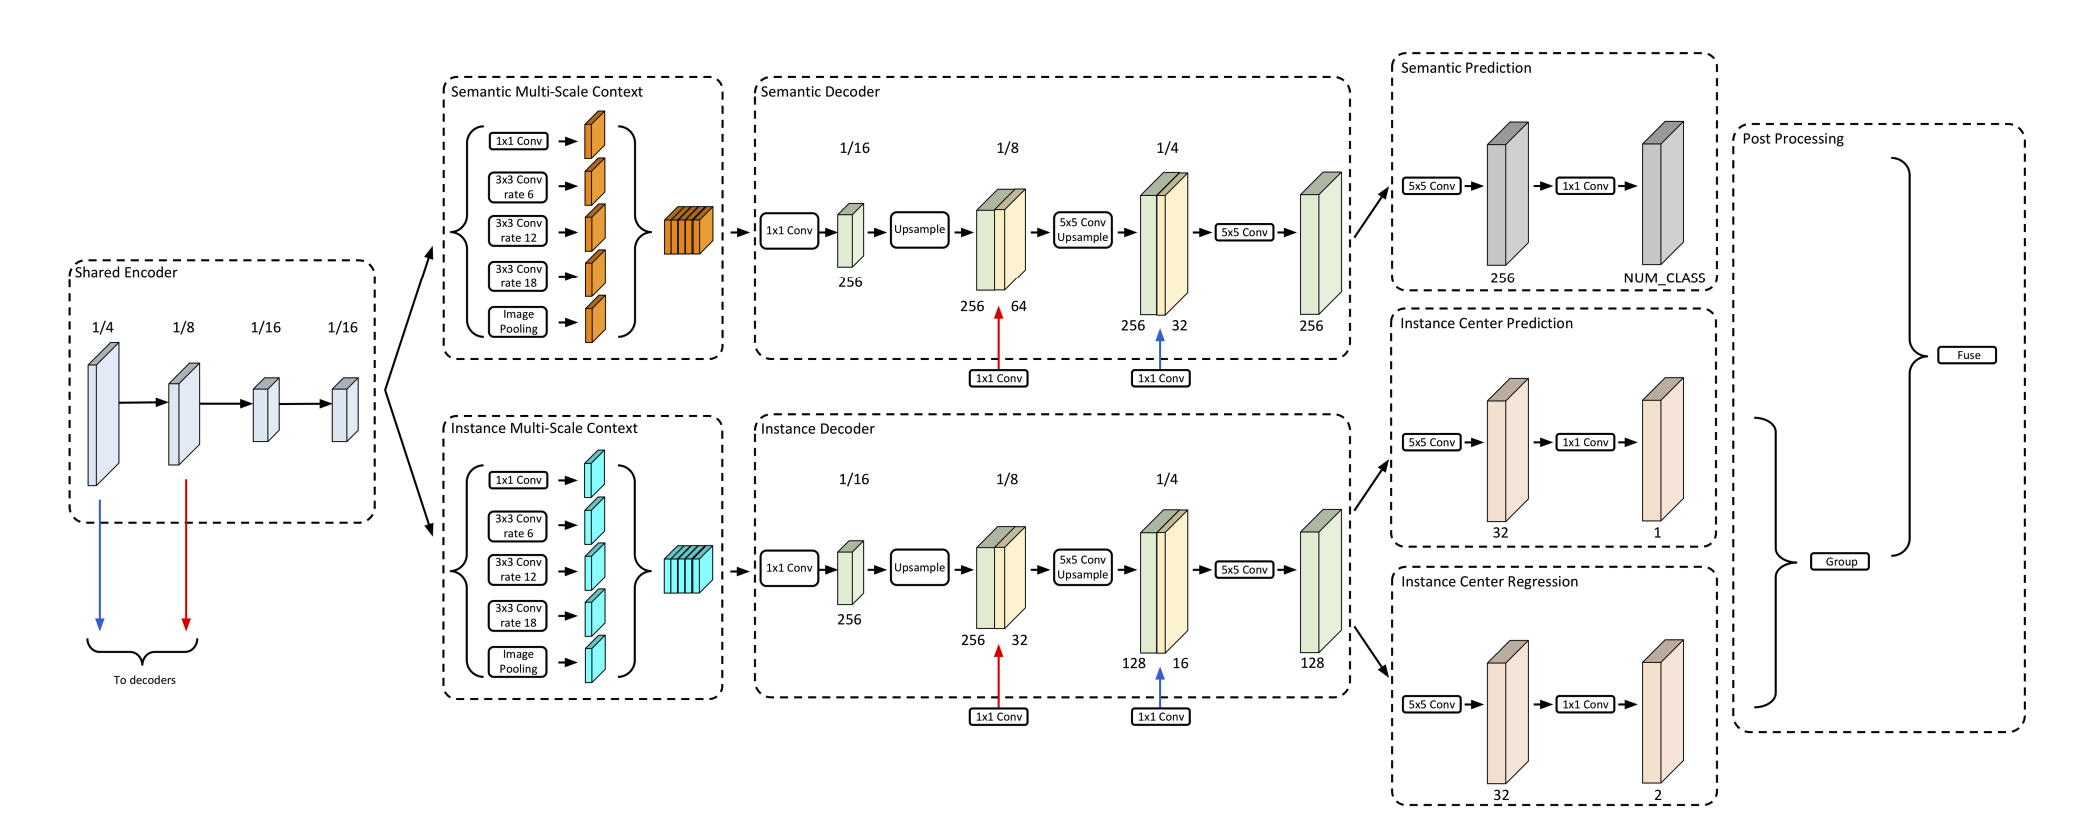
\includegraphics[width=18cm, trim={1cm 0 1cm 0.5cm},clip]{latex/Images/panoptic_deeplab.png}}
\caption{Panoptic DeepLab architecture}
\label{fig:panoptic_deeplab_arch}
\end{figure*}

%\newpage
%\newpage

\section{Panoptic FPN}
\label{app:fpn}

Figure \ref{fig:modifications} shows the modifications to the original backbone architectures used by the detectron2 library. Figure \ref{fig:pre-resnetmod} shows a demonstration of the trained model based on a modified ResNet50 backbone. 

\begin{figure*}[htbp]
\centering
\fbox{\includegraphics[width=8.5cm, height=14cm]{latex/Images/mods.jpg}}
\caption{Modifications to the backbones of a Panoptic FPN architecture}
\label{fig:modifications}
\end{figure*}

\begin{figure*}[htbp]
\centering
\fbox{\includegraphics[width=14cm, trim={1cm 0 1cm 0.5cm},clip]{latex/Images/app1.jpg}}
\caption{Predicted panoptic segmentation based on Panoptic FPN with a modified ResNet50 backbone}
\label{fig:pre-resnetmod}
\end{figure*}

%\section{Miscellaneous Information}

%The rest of the information in this format template has been adapted from CVPR 2020 and provides guidelines on the lower-level specifications regarding the paper's format.

%\subsection{Language}

%All manuscripts must be in English.


%\subsection{Paper length}
%Papers, excluding the references section,
%must be no longer than six pages in length. The references section
%will not be included in the page count, and there is no limit on the
%length of the references section. For example, a paper of six pages
%with two pages of references would have a total length of 8 pages.

%-------------------------------------------------------------------------
%\subsection{The ruler}
%The \LaTeX\ style defines a printed ruler which should be present in the
%version submitted for review.  The ruler is provided in order that
%reviewers may comment on particular lines in the paper without
%circumlocution.  If you are preparing a document using a non-\LaTeX\
%document preparation system, please arrange for an equivalent ruler to
%appear on the final output pages.  The presence or absence of the ruler
%should not change the appearance of any other content on the page.  The
%camera ready copy should not contain a ruler. (\LaTeX\ users may uncomment
%the \verb'\cvprfinalcopy' command in the document preamble.)  Reviewers:
%note that the ruler measurements do not align well with lines in the paper
%--- this turns out to be very difficult to do well when the paper contains
%many figures and equations, and, when done, looks ugly.  Just use fractional
%references (e.g.\ this line is $095.5$), although in most cases one would
%expect that the approximate location will be adequate.

%\subsection{Mathematics}

%Please number all of your sections and displayed equations.  It is
%important for readers to be able to refer to any particular equation.  Just
%because you didn't refer to it in the text doesn't mean some future reader
%might not need to refer to it.  It is cumbersome to have to use
%circumlocutions like ``the equation second from the top of page 3 column
%1''.  (Note that the ruler will not be present in the final copy, so is not
%an alternative to equation numbers).  All authors will benefit from reading
%Mermin's description of how to write mathematics:
%\url{http://www.pamitc.org/documents/mermin.pdf}.

%Finally, you may feel you need to tell the reader that more details can be
%found elsewhere, and refer them to a technical report.  For conference
%submissions, the paper must stand on its own, and not {\em require} the
%reviewer to go to a techreport for further details.  Thus, you may say in
%the body of the paper ``further details may be found
%in~\cite{Authors14b}''.  Then submit the techreport as additional material.
%Again, you may not assume the reviewers will read this material.

%Sometimes your paper is about a problem which you tested using a tool which
%is widely known to be restricted to a single institution.  For example,
%let's say it's 1969, you have solved a key problem on the Apollo lander,
%and you believe that the CVPR70 audience would like to hear about your
%solution.  The work is a development of your celebrated 1968 paper entitled
%``Zero-g frobnication: How being the only people in the world with access to
%the Apollo lander source code makes us a wow at parties'', by Zeus \etal.

%You can handle this paper like any other.  Don't write ``We show how to
%improve our previous work [Anonymous, 1968].  This time we tested the
%algorithm on a lunar lander [name of lander removed for blind review]''.
%That would be silly, and would immediately identify the authors. Instead
%write the following:
%\begin{quotation}
%\noindent
   %We describe a system for zero-g frobnication.  This
   %system is new because it handles the following cases:
   %A, B.  Previous systems [Zeus et al. 1968] didn't
   %handle case B properly.  Ours handles it by including
   %a foo term in the bar integral.

   %...

   %The proposed system was integrated with the Apollo
   %lunar lander, and went all the way to the moon, don't
   %you know.  It displayed the following behaviours
   %which show how well we solved cases A and B: ...
%\end{quotation}
%As you can see, the above text follows standard scientific convention,
%reads better than the first version, and does not explicitly name you as
%the authors.  A reviewer might think it likely that the new paper was
%written by Zeus \etal, but cannot make any decision based on that guess.
%He or she would have to be sure that no other authors could have been
%contracted to solve problem B.
%\medskip


%\subsection{Miscellaneous}

%\noindent
%Compare the following:\\
%\begin{tabular}{ll}
% \verb'$conf_a$' &  $conf_a$ \\
% \verb'$\mathit{conf}_a$' & $\mathit{conf}_a$
%\end{tabular}\\
%See The \TeX book, p165.

%The space after \eg, meaning ``for example'', should not be a
%sentence-ending space. So \eg is correct, {\em e.g.} is not.  The provided
%\verb'\eg' macro takes care of this.

%When citing a multi-author paper, you may save space by using ``et alia'',
%shortened to ``\etal'' (not ``{\em et.\ al.}'' as ``{\em et}'' is a complete word.)
%However, use it only when there are three or more authors.  Thus, the
%following is correct: ``
   %Frobnication has been trendy lately.
   %It was introduced by Alpher~\cite{Alpher02}, and subsequently developed by
   %Alpher and Fotheringham-Smythe~\cite{Alpher03}, and Alpher \etal~\cite{Alpher04}.''


%this is first developed by Kirillov \etal~\cite{kirillov2019panoptic}. 


%This is incorrect: ``... subsequently developed by Alpher \etal~\cite{Alpher03} ...''
%because reference~\cite{Alpher03} has just two authors.  If you use the
%\verb'\etal' macro provided, then you need not worry about double periods
%when used at the end of a sentence as in Alpher \etal.

%For this citation style, keep multiple citations in numerical (not
%chronological) order, so prefer \cite{Alpher03,Alpher02,Authors14} to
%\cite{Alpher02,Alpher03,Authors14}.


%------------------------------------------------------------------------
%\subsection{Formatting your paper}

%All text must be in a two-column format. The total allowable width of the
%text area is $6\frac78$ inches (17.5 cm) wide by $8\frac78$ inches (22.54
%cm) high. Columns are to be $3\frac14$ inches (8.25 cm) wide, with a
%$\frac{5}{16}$ inch (0.8 cm) space between them. The main title (on the
%first page) should begin 1.0 inch (2.54 cm) from the top edge of the
%page. The second and following pages should begin 1.0 inch (2.54 cm) from
%the top edge. On all pages, the bottom margin should be 1-1/8 inches (2.86
%cm) from the bottom edge of the page for $8.5 \times 11$-inch paper; for A4
%paper, approximately 1-5/8 inches (4.13 cm) from the bottom edge of the
%page.

%-------------------------------------------------------------------------
%\subsection{Margins and page numbering}

%All printed material, including text, illustrations, and charts, must be kept
%within a print area 6-7/8 inches (17.5 cm) wide by 8-7/8 inches (22.54 cm)
%high.



%-------------------------------------------------------------------------
%\subsection{Type-style and fonts}

%Wherever Times is specified, Times Roman may also be used. If neither is
%available on your word processor, please use the font closest in
%appearance to Times to which you have access.

%MAIN TITLE. Center the title 1-3/8 inches (3.49 cm) from the top edge of
%the first page. The title should be in Times 14-point, boldface type.
%Capitalize the first letter of nouns, pronouns, verbs, adjectives, and
%adverbs; do not capitalize articles, coordinate conjunctions, or
%prepositions (unless the title begins with such a word). Leave two blank
%lines after the title.

%AUTHOR NAME(s) and AFFILIATION(s) are to be centered beneath the title
%and printed in Times 12-point, non-boldface type. This information is to
%be followed by two blank lines.

%The ABSTRACT and MAIN TEXT are to be in a two-column format.

%MAIN TEXT. Type main text in 10-point Times, single-spaced. Do NOT use
%double-spacing. All paragraphs should be indented 1 pica (approx. 1/6
%inch or 0.422 cm). Make sure your text is fully justified---that is,
%flush left and flush right. Please do not place any additional blank
%lines between paragraphs.

%Figure and table captions should be 9-point Roman type as in
%Figures~\ref{fig:onecol} and~\ref{fig:short}.  Short captions should be centred.

%\noindent Callouts should be 9-point Helvetica, non-boldface type.
%Initially capitalize only the first word of section titles and first-,
%second-, and third-order headings.

%FIRST-ORDER HEADINGS. (For example, {\large \bf 1. Introduction})
%should be Times 12-point boldface, initially capitalized, flush left,
%with one blank line before, and one blank line after.

%SECOND-ORDER HEADINGS. (For example, { \bf 1.1. Database elements})
%should be Times 11-point boldface, initially capitalized, flush left,
%with one blank line before, and one after. If you require a third-order
%heading (we discourage it), use 10-point Times, boldface, initially
%capitalized, flush left, preceded by one blank line, followed by a period
%and your text on the same line.

%-------------------------------------------------------------------------
%\subsection{Footnotes}

%Please use footnotes\footnote {This is what a footnote looks like.  It
%often distracts the reader from the main flow of the argument.} sparingly.
%Indeed, try to avoid footnotes altogether and include necessary peripheral
%observations in
%the text (within parentheses, if you prefer, as in this sentence).  If you
%wish to use a footnote, place it at the bottom of the column on the page on
%which it is referenced. Use Times 8-point type, single-spaced.


%-------------------------------------------------------------------------
%\subsection{References}

%List and number all bibliographical references in 9-point Times,
%single-spaced, at the end of your paper. When referenced in the text,
%enclose the citation number in square brackets, for
%example~\cite{Authors14}.  Where appropriate, include the name(s) of
%editors of referenced books.

%\begin{table}
%\begin{center}
%\begin{tabular}{|l|c|}
%\hline
%Method & Frobnability \\
%\hline\hline
%Theirs & Frumpy \\
%Yours & Frobbly \\
%Ours & Makes one's heart Frob\\
%\hline
%\end{tabular}
%\end{center}
%\caption{Results.   Ours is better.}
%\end{table}

%-------------------------------------------------------------------------
%\subsection{Illustrations, graphs, and photographs}

%All graphics should be centered.  Please ensure that any point you wish to
%make is resolvable in a printed copy of the paper.  Resize fonts in figures
%to match the font in the body text, and choose line widths which render
%effectively in print.  Many readers (and reviewers), even of an electronic
%copy, will choose to print your paper in order to read it.  You cannot
%insist that they do otherwise, and therefore must not assume that they can
%zoom in to see tiny details on a graphic.

%When placing figures in \LaTeX, it's almost always best to use
%\verb+\includegraphics+, and to specify the  figure width as a multiple of
%the line width as in the example below
%{\small\begin{verbatim}
   %\usepackage[dvips]{graphicx} ...
   %\includegraphics[width=0.8\linewidth]
                   %{myfile.eps}
%\end{verbatim}
%}


%-------------------------------------------------------------------------
%\subsection{Color}

%Please refer to the author guidelines on the CVPR 2020 web page for a discussion
%of the use of color in your document.

%------------------------------------------------------------------------

%-------------------------------------------------------------------------



\end{document}
